
\chapter{Newspaper Mail
} 
Few complete newspapers illustrating the 1d. rate have survived. A rarity! Photo-cert: PFSA. This edition includes at top left front an advertisement for the purchase of 50 copies of the newspaper for 2nd & 6th February (which a manuscript endorsement in another hand records "these copies contain the correspondence between Mr Baines and Dr Livingstone, the Foreign and Colonial Offices"). Note: At this time Thomas Baines had returned to the Cape in disgrace at having been dismissed by Livingstone from the Zambezi expedition accused of theft. By this correspondence Baines was obviously keeping his mother informed on what had been presented in the local press regarding the charges brought against him. The newspaper also records under the jottings of "The Hermit of Adderley Street"... "One of the most painful histories I have read for a long time is that detailed in the lately published Baines correspondence..." (highlighted by Baines in red pen). A rare newspaper franking with the added interest of it's Africana historical significance. .rsrgri/031	
Price: \$ 5080

\begin{figure*}

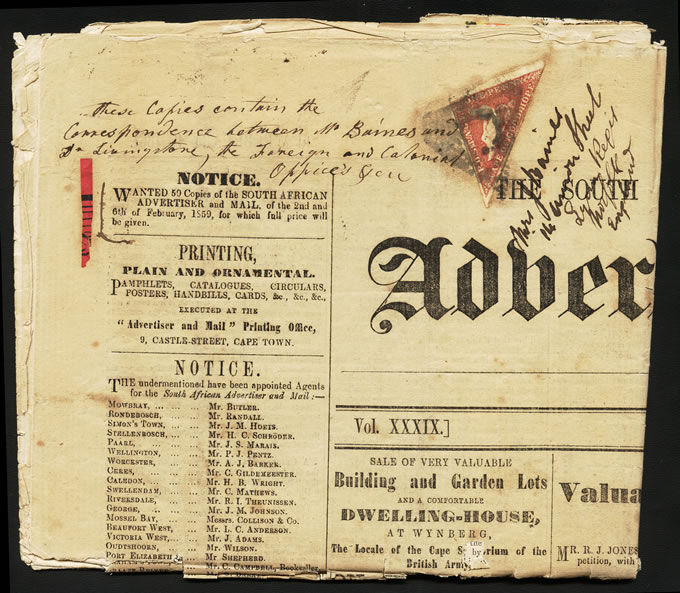
\includegraphics[width=1.0\textwidth]{../cape-of-good-hope/newspaper-triangular.jpg}
\caption{
1861 COMPLETE NEWSPAPER being the February 9th edition of "The South African Advertiser and Mail" addressed in the hand of artist Thomas Baines to his mother Mrs J Baines in Lynn Regis, England, at the 1d NEWSPAPER RATE. This special postage rate paid by single 1d deep rose-red triangular (SG 5b), clear to large margins all around excepting just touching along bottom right. }
\end{figure*}

<p class="small">Johnson 2009</p><div style="clear:both"></div>

 
  